\chapter{Fundamentos básicos}

Este capitulo apresenta os principais conceitos e definições necessários para o entendimento deste trabalho. A seção 2.1 apresenta definições de sistemas multiagentes.
A seção 2.2 apresenta uma breve explicação sobre a arquitetura da plataforma JAMA, bem como o seu funcionamento.
A seção 2.3 contém uma breve introdução sobre dependabilidade.
Por fim, a seção 2.4 tem um texto expondo o funcionamento do JAMA, bem como a sua arquitetura.

\section{Sistemas Multiagentes}

\subsection{Inteligência artificial}

Antes de explicarmos o conceito de sistemas multiagentes (SMA), é necessário mostrar conceitos que são base para o entendimento de SMA. Inicia-se apresentando alguns conceitos de Inteligencia Artificial (IA). De acordo com~\cite{poole98} identificamos que a definição de IA pode variar em duas dimensões principais. Usando a definição de sistemas computacionais que agem racionalmente temos:

\begin{quote}
\emph{Computational Intelligence is the study of the design of intelligent agents.}
\end{quote}

Nessa definição, é importante ressaltar que o agente é uma entidade que atua racionalmente, esperando-se que essa racionalidade e outras características o diferencie de simples programas.

Com o crescimento dos estudos relacionado a este campo, a inteligência artificial ganhou várias áreas de atuação e resolução de problemas no nosso cotidiano. Um dos problemas é a necessidade de executar aplicações que resolvem problemas de alta complexidade. Essas aplicações podem exigir um hardware muito caro para a execução, ou então pode-se usar a abordagem de distribuí-la em vários computadores que dividem a sua execução. É justamente onde entra a inteligência artificial distribuída: São sistemas que são compostos por vários agentes coletivos, ou seja, distribuem o trabalho uns com os outros. Cada agente pode possuir uma capacidade diferente, sendo possível realizar a tarefa de modo paralelo. 

\subsection{Agente}

De acordo com~\cite{novig95}, agentes são entidades (reais ou virtuais) que funcionam de forma autônoma em um ambiente, ou seja, não necessitam de intervenção humana para realizar processamento. Esse ambiente de funcionamento do agente geralmente contém vários outros agentes e é possível a comunicação entre eles através do ambiente por meio de troca de mensagens.

Em geral o funcionamento de agentes acontece de forma a perceberem o ambiente em que estão por meio de sensores, fazem análises com base nessa interação inicial e por fim podem agir sobre o ambiente de forma a modifica-lo por meio de efetuadores. A figura~\ref{fig:agente-basico} apresenta um resumo do que foi dito.

\begin{figure}
	\centering
	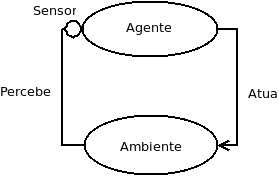
\includegraphics[scale=0.75]{images/agente-basico.png}
	\caption{Esquematização do funcionamento básico de um agente em um ambiente.}
	\label{fig:agente-basico}
\end{figure}

Agentes racionais seguem o princípio de racionalidade básico: sempre objetivam suas ações pela escolha da melhor ação possível segundo seus conhecimentos. Logo é possível inferir que a ação de um agente nem sempre alcança o máximo desempenho, sendo desempenho o parâmetro definido para medir o grau de sucesso da ação de um agente com base nos seus objetivos.

Como dito anteriormente, agentes estão presentes em um ambiente. O agente não tem controle total do ambiente, ele pode no máximo influenciá-lo com a sua atuação. Podemos separar ambientes em classes: Software, Físico e Relidade virtual (simulação de ambientes reais em software). De acordo com~\cite{wooldridge04} temos, em geral, ambientes tem propriedades inerentes que dizem respeito ao seu funcionamento:

\begin{itemize}
	\item Observável: Neste tipo de ambiente, os sensores dos agentes conseguem ter percepção completa do ambiente. Por exemplo, um sensor de movimento consegue ter visão total em um ambiente aberto.
	\item Determinística: O próximo estado do ambiente é sempre conhecido dado o estado atual do ambiente e as ações dos agentes. O oposto do ambiente determinístico é o estocástico, quando não temos certeza do estado do ambiente. Por exemplo, agentes dependentes de eventos climáticos.
	\item Episódico: A experiência do agente é dividida em episódios, onde cada episódio é a percepção do agente e a sua ação.
	\item Sequêncial: A ação tomada pelo agente pode afetar o estado do ambiente e ocasionar na mudança de estado
	\item Estático: O ambiente não é alterado enquanto um agente escolhe uma ação.
	\item Discreto: Existe um número definido de ações e percepções do agente para o ambiente em cada turno.
	\item Contínuo: As percepções e ações de um agente modificam-se em um espectro contínuo de valores. Por exemplo, temperatura de um sensor muda de forma contínua.
\end{itemize}

Na tabela~\ref{lista_agentes} mostramos alguns exemplos de agentes, apresentando as suas características já discutidas nesse trabalho.

\begin{table}
	\caption{Listagem de sistemas multiagentes com propriedades de medida de performance, ambiente, atuadores e sensores}
	\begin{tabular}{|p{3cm} | p{3cm} | p{2cm}| p{3cm} | p{3cm} |}
		\hline
		\textbf{Tipo de agente}	& \textbf{Medida de performance} & \textbf{Ambiente} & \textbf{Atuadores}  & \textbf{Sensores}	\\
		\hline
		Sensores de estacionamento	& Avarias no veículo & Carro e garagens & Freio do carro, controle de velocidade & Sensor de proximidade	\\
		\hline
		Jogos com oponente computador	& Quantidade de vitórias &	Software & Realizar jogada & Percepção do tabuleiro	\\
		\hline
		Agentes hospitalares		& Saúde do paciente & Paciente, ambiente médico & Diagnósticos & Entrada de sintomas do paciente	\\
		\hline
	\end{tabular}
	\label{lista_agentes}
\end{table}
 
A primeira linha da tabela~\ref{lista_agentes} é apresentado um exemplo de um agente atuando em um veículo como um sensor de estacionamento. Responsável por auxiliar o motorista no ato de estacionar o carro, o seu ambiente é da classe físico (considerando o carro e o ambiente onde está o carro). Seu sensor de proximidade é a percepção do ambiente e caso detecte que está próximo de um obstáculo pode atuar nos freios dos carros diminuindo a velocidade e evitando colisões. Avarias no carro podem indicar um mal funcionamento do sensor.

A segunda linha da tabela é apresentado u exemplo de agente atuando em um jogo qualquer. Esse ambiente é dito dinâmico, pois a cada jogada de um oponente (real ou não), o agente irá analisar a jogada feita pelo seu oponente, irá calcular sua próxima jogada e irá realizá-la. O objetivo principal do agente é a vitória. O ambiente que o agente atua é um software e o seu atuador é um algum mecanismo que permite que ele realize a jogada. O sensor é o mecanismo no qual o agente irá perceber a jogada realizada pelo oponente.

Por fim, última linha da tabela~\ref{lista_agentes} expõe um exemplo de um agente médico atuando em um ambiente estático um paciente. Esse ambiente é dito estático por que não será alterado pelo agente nesse exemplo, mas podendo ser diferente dependendo da aplicação. O objetivo principal é monitorar a saúde do paciênte, logo a medida de performance será a aproximação ou não do diagnóstico médico. Seu atuador não será diretamente no ambiente (corpo humano), será na forma de relatórios médicos e seus sensores podem variar de acordo com a doença a ser monitorada.

Conforme podemos encontrar em~\cite{wooldridge04}, podemos definir algumas noções gerais de agentes. A primeira, chamada de noção fraca, contém a maior parte dos agentes. Ela compreende os aspectos de \emph{reatividade}, \emph{proatividade} e \emph{habilidade social}. O conceito de reatividade  está ligado com o agente perceber o ambiente e reagir. Proatividade é a característica do agente tomar a iniciativa e agir sem a necessidade de nenhum estímulo. Habilidade social é a capacidade de interação com outros agentes.

Já a noção forte de agente envolve os seguintes aspectos: , veracidade, benevolência
\begin{itemize}
	\item Mobilidade: O Agente deve pode mover-se no ambiente, por exemplo, em uma rede.
	\item Veracidade: Agente não comunica informações falsas.
	\item Benevolência: Agente ajudará os outros.
	\item Racionalidade: O agente não irá agir de forma a impedir a realização de seus objetivos.
	\item Cooperação: O agente coopera com o usuário.
\end{itemize}

\subsection{Arquitetura de agentes}

A arquitetura de agentes varia de acordo com a complexidade da sua autonomia, ou seja, com a capacidade de reagir aos estímulos do ambiente. Conforme verificado no livro de ~\cite{novig95}, os tipos de arquitetura são: orientadas à tabela, reflexiva simples, reflexiva baseado em modelo, baseada em objetivo, baseada em utilidade.

A primeira arquitetura a ser explorada é o agente orientado à tabelas. Todas as ações dos agentes dessa arquitetura são conhecidas e estão gravadas em uma tabela. Assim, quando o agente receber o estímulo ele já terá a ação a ser tomada previamente gravada em sua memória. Logo para construir esse tipo de agente, fica claro que além de saber todas percepções possívels, será necessário definir ações apropriadas para todas. Isso levará a tabelas muito complexas e o tamanho pode facilmente passar a ordem de milhões dependendo do número de entradas.

A arquitetura reflexiva simples é um dos tipos mais simples de agente. Nele, o agente seleciona a ação com base unicamente na percepção atual, desconsiderando assim uma grande tabela de decisões. A decisão é tomada com base de regras condição-ação: Se uma condição ocorrer, uma ação será tomada. Por exemplo, vamos supor um agente médico que determina o diagnóstico de uma doença no paciente caso exista alguma anomalia no organismo (Por exemplo, paciente com febre). Uma condição-ação poderia ser:

if anomalia-organismo then diagnóstico-médico

Esse tipo de agente é bastante simples, o que é uma vantagem comparado à arquitetura de tabela. Porém, essa abordagem requer um ambiente totalmente observável, visto que esse tipo de agente possui uma inteligência bastante limitada. No exemplo do agente médico existem diversas maneiras de se detectar uma anomalia no organismo do paciente, seria necessário conhecer todas as formas para usarmos uma abordagem reativa simples.

A arquitetura reflexiva baseada em modelos funciona de maneira similar a anterior. Nessa abordagem, é levado em conta a parte do ambiente que não é visível neste momento. E para saber o ``momento atual'' de um agente, é necessário guardar a informação de estado consigo. Para atualizar o estado do agente, é necessário conhecer como o mundo desenvolve-se independente do agente (no caso do exemplo, como o organismo funciona) e é necessário saber as ações dos agentes no ambiente. Esses dois conhecimentos do ambiente são chamados de \textbf{modelo do mundo}. O agente que usa esse tipo de abordagem é chamado de agente baseado em modelo.

Na arquitetura reflexiva baseada em objetivo, as ações do agente são tomadas apenas se o aproximam de alcançar um objetivo. Para isso, será necessário algo além do estado atual do ambiente: Será necessário informações do objetivo a ser atingido. Assim o agente pode combinar as informações do estado e o objetivo para determinar se deve ou não agir sobre o ambiente. Essa arquitetura porém é obviamente mais complexa e de certa forma ineficiente. Porém ela permite uma maior flexibilização das ações em determinados ambientes, visto que suas decisões são representadas de forma explícita e podem ser modificadas. É interessante notar que esse tipo de arquitetura não trata ações com objetivos conflitantes.

E por fim, a arquitetura reflexiva baseada em utilidade não utiliza apenas objetivos para realizar a próxima decisão, mas dá ao agente a capacidade de fazer comparações sobre o estado do ambiente e as ações a serem tomadas: Quais delas são mais baratas, confiáveis, baratas, rápidas do que as outras. A capacidade de avaliação do agente chama-se função de utilidade, que mapeia uma sequência de estados em um número real que determina o grau de utilidade. Esse mecanismo possibilita a decisão racional de escolha entre vários objetivos conflitantes. Por exemplo, escolher entre um objetivo mais barato ao invés de escolher entre o mais rápido.

\subsection{Sistemas Multiagentes}

Sistemas multiagentes são sistemas compostos por vários agentes capazes de se comunicar, possuindo uma linguagem de alto nível para isso. O agente deve ser conhecimento para realizar uma determinada tarefa e pode ou não cooperar com outros agentes para realizá-la.

Fica claro nessa definição que sistemas multiagentes

De acordo com~\cite{sarmento11}, podemos encontrar as seguintes características principais de ambientes em SMAs:
\begin{itemize}
	\item Ambientes SMAs fornecem protocolos específicos para comunicação e interação. Cada ambiente tem as suas particularidades: Alguns são em uma única máquina, outros são compartilhados com o mundo real e outros são distribuídos. Cabe a cada ambiente definir um protocolo onde todos agentes devem obedecer para comunicar-se.
	\item SMAs são tipicamente abertos.
	\item SMAs contém agentes que são autônomos e individualistas.
\end{itemize}

\section{Dependabilidade}

Antes de falar em dependabilidade, são necessárias algumas definições.

A definição original de dependabilidade de software é a habilidade de um sistema prover um serviço ao qual seja possível justificadamente confiar. Uma outra definição alternativa é a dependabilidade de um sistema é a habilidade de evitar falhas que são mais frequentes e mais graves do que o aceitável.

Dependabilidade é uma área que vem desenvolvendo seus estudos de forma crescente ao longo dos anos. De acordo com~\cite{algirdas04}, o conceito de dependabilidade abrange uma série de principais atributos que a integram.

O primeiro deles é disponibilidade, onde um serviço deve estar o disponível o máximo de tempo possível. A confiabilidade garante que o serviço usado é sempre confiável.

A segurança é a garantia de não haver consequências catastróficas para o ambiente no uso do serviço. Integridade garante não alteração nas propriedades. Manutenibilidade é a garantia que é possível mudanças e reparos no sistema provedor do serviço.

Alguns atributos são muito próximos da segurança da informação, como por exemplo a confidencialidade, que é a capacidade de não prover informação para entidades desconhecidas. Outros atributos são, na verdade, uma composição com a segurança. Por exemplo a integridade e disponibilidade. Integridade com acessos não autorizados e disponibilidade apenas para acessos autorizados. A figura~\ref{fig:dependabilidade-seguranca} sintetiza o que foi dito, mostrando os atributos em comum das duas áreas.

\begin{figure}
	\centering
	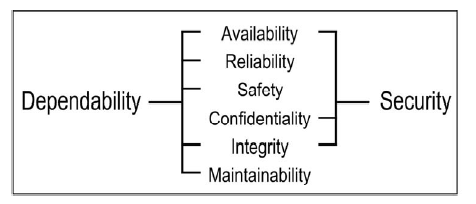
\includegraphics[scale=0.75]{images/dependabilidade-seguranca.png}
	\caption{Dependabilidade, segurança e seus atributos em comum.~\cite{algirdas04}}
	\label{fig:dependabilidade-seguranca}
\end{figure}

Dado que sistemas começam a ser modelados a partir de especificações de componentes, os desafios de dependabilidade hoje para estudos futuros são muitos. O primeiro deles é determinar precisamente a qualidade desses atributos de forma precisa, sabendo que são especificados de forma imprecisa. É necessário também determinar em que medida e quais restrições as propriedades emergentes podem ser derivadas das propriedades de um sistema. E dado um conjunto de propriedades, quais delas são previsíveis.

Mais especificamente, em um sistema multiagente, é a propriedade que podemos medir sobre a confiança que podemos mensurar em um agente dado que ele roda em um ambiente descentralizado. Devido a complexidade do ambiente, existem diversos desafios de acordo com~\cite{hoffman08} no projeto desse ambiente. Em~\cite{algirdas04} são definidos as principais propriedades relacionadas a dependabilidade, sendo um dos objetivos deste trabalho a identificação destas propriedades na plataforma JAMA.

Alguns conceitos mais elementares em dependabilidade podem parecer sinônimos, porém tem significados distintos. Erros, faltas e falhas possuem os seguintes significados, todas de acordo com~\cite{algirdas04}:
\begin{itemize}
	\item Falta (~\emph{fault}) - Ocorre quando um serviço disponível em um sistema é entregue de maneira diferente do esperado.
	\item Erro (~\emph{error}) - A diferença entre o serviço entregue e o serviço esperado é chamado de erro.
	\item Falha (~\emph{failure}) - É a manifestação do erro para o usuário do sistema seja por mensagens de erro personalizadas, ~\emph{stack trace}, dentre outros.
\end{itemize}

Em geral, faltas que podem prejudicar o funcionamento do sistema durante seu uso são classificadas em oito classes, podendo ser combinadas uma a uma gerando um total de 256 faltas. Como nem todas as combinações são possíveis, verifica-se em~\cite{algirdas04} as principais combinações de falhas mapeadas.

A primeira das principais faltas é durante fase de criação do software. Elas ocorrem durante a codificação do sistema, e podem ocorrer nas seguintes etapas: Desenvolvimento do sistema, manutenção do sistema ou na geração incorreta de procedimentos para uso ou manutenção do sistema.

Outra principal falta pode ocorrer nos limites do sistema, ou seja, o limite entre o sistema a ser desenvolvido e o mundo real ao qual ele será aplicado. As falhas nessa classe podem ocorrer na parte interna do sistema, causado na parte interna da fronteira do sistema, ou pode ser originado na parte externa do sistema, mais especificamente pela interação com o sistema.

As faltas fenomenológicas são causadas por fenômenos naturais (falta de energia, alagamento, dentre outros) que podem danificar o sistema, ou então causadas pela ação do homem, por exemplo, incêndios, \emph{hardware} danificado, dentre outros.

As faltas com objetivo são originadas com uma inserção de um componente estranho no sistema. Essa falha pode ser ocasionada objetivando a danificação do sistema, por exemplo, a introdução de códigos maliciosos prejudiciais ao sistema, assim como é possível também ocorrer de forma não maliciosa.

Faltas por capacidade são faltas ocorridas com a interação com o sistema, seja na manutenção, desenvolvimento, ou ação do usuário. Podem ocorrer no sistema de forma acidental, por exemplo, uma introdução de um dado não suportado pelo sistema. Mais frequentemente, faltas por capacidade ocorrem pela falta de capacidade profissional por parte das pessoas autorizadas a realizar manutenção do sistema.

Por fim, as faltas persistentes podem ser as mais danosas ao sistema e são caracterizadas pelo tempo de permanência no sistema. Classificadas como transientes ou persistentes, ocorrem em conjunto com outras falhas.

A figura~\ref{fig:algirdas-fault} sintetiza todas as classes descritas nessa seção, bem como lista as principais combinações de classes existentes.
As imagens~\ref{fig:dependabilidade-combinacao} e~\ref{fig:dependabilidade-matriz} combinam as classes de falha e mostra uma visualização em forma de matriz e árvore, respectivamente.

\begin{figure}
	\centering
	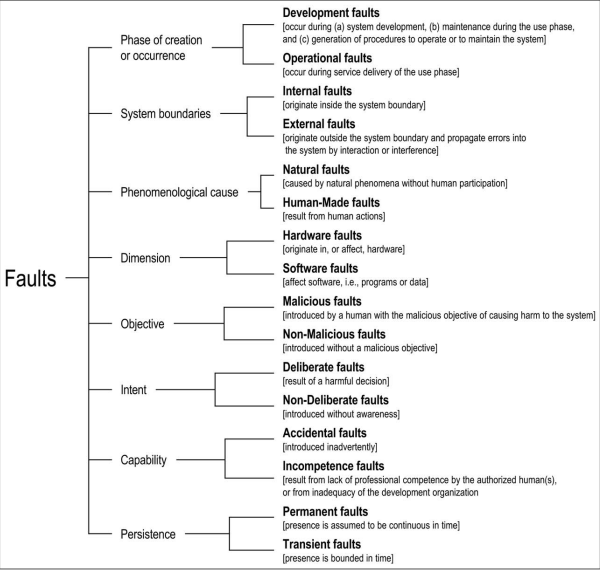
\includegraphics[scale=0.5]{images/algirdas-fault.png}
	\caption{As classes de faltas elementares.~\cite{algirdas04}}
	\label{fig:algirdas-fault}
\end{figure}

\begin{figure}
	\centering
	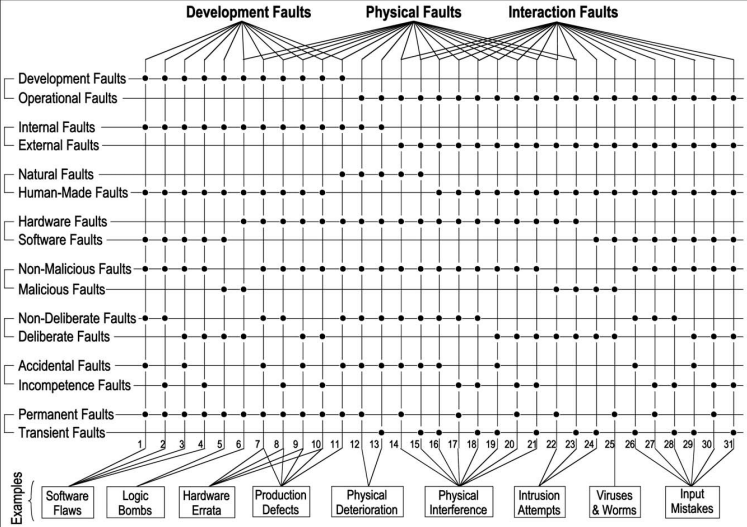
\includegraphics[scale=0.6]{images/dependabilidade-combinacao.png}
	\caption{Combinação de classes de faltas elementares em forma de matriz.~\cite{algirdas04}}
	\label{fig:dependabilidade-combinacao}
\end{figure}

\begin{figure}
	\centering
	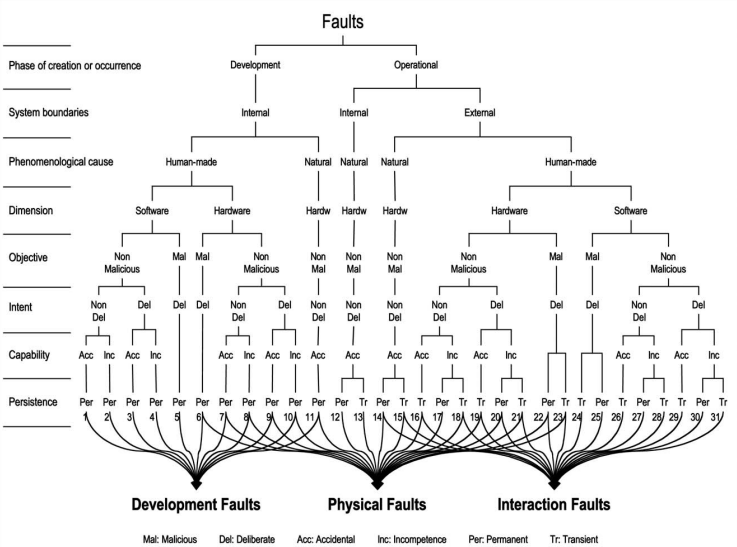
\includegraphics[scale=0.6]{images/dependabilidade-matriz.png}
	\caption{Combinação de classes de faltas elementares em forma de árvore.~\cite{algirdas04}}
	\label{fig:dependabilidade-matriz}
\end{figure}

Em um sistema P2P, a dificuldade de medir o grau de dependabilidade é bastante complexo, pois é necessário determinar propriedades que são, em sua grande maioria, sensíveis ao contexto. Em cada sistema é possível medir a dependabilidade tendo em vista características que, em um outro sistema ou contexto, essas características não tem tanta importância.

É importante notar que a medida de dependabilidade pode mudar de acordo com a arquitetura utilizada no sistema P2P. Por exemplo, redes totalmente descentralizadas podem ser mais resistentes à ataques de negação de serviço do que redes com algum tipo de localização centralizada.

De acordo com~\cite{walkerdine02}, são levantadas as principais propriedades de dependabilidades para sistemas P2P. No mesmo trabalho, eles dividem as propriedades em duas categorias: Arquiteturais e emergentes. Propriedades arquiteturais são diretamente afetadas pela arquitetura. Propriedades emergentes surgem com o uso da arquitetura.

As principais propriedades de arquitetura são:
\begin{itemize}
	\item Confiança - A confiabilidade medida de um sistema.
	\item Escalabilidade - Capacidade de um sistema manter o mesmo desempenho dado que o número de acessos aumenta ou diminui.
	\item Segurança - O nível de segurança dentro de um sistema representa sua capacidade de se proteger contra uma intrusão, seja ela acidental ou proposital.
	\item Capacidade de sobrevivência - Capacidade de um sistema para cumprir a sua missão em tempo hábil, na presença de ataques, falhas ou acidentes.
	\item Segurança - Capacidade do sistema em operar sem nenhuma falha catastrófica.
	\item Manutenibilidade - Capacidade de modificação de um sistema, considerando que ele já está entregue e que está em pleno funcionamento, ou seja, em produção.
	\item Responsabilidade - A garantia em um sistema que são aplicadas regras de responsabilidade social com os dados dos usuários.
	\item Disponibilidade - A garantia de que um sistema estará operacional e capaz de entregar as requisições feitas na maior parte do tempo.
	\item Tolerância a Falhas - a capacidade de um sistema para continuar dando um serviço correto após a manifestação de uma falhas.~\cite{sommerville95}
	\item Independência política e jurídica - Medida de quão fácil é encerrar o funcionamento de um sistema.
	\item Integridade dos dados - Capacidade do sistema de manter a integridade dos dados que são armazenados e manipulados durante o seu funcionamento.
	\item Conectividade dinâmica - A arquitetura garante a conectividade dinâmica de pares dentro de um sistema, onde nós entram e saem da rede se causar nenhuma falha catastrófica.
	\item Descoberta de pares - A arquitetura garante mecanismos seguros usados para descobrirem outros pares na rede.
	\item Anonimato - Capacidade da rede de garantir o anonimato de usuários ou os dados trafegados na rede.
discovering other peers on the network.
	\item Balanceamento de carga - A carga total do sistema é distribuído igualmente entre todos os pares da rede, garantindo que alguns pares não são sobrecarregados com processamento excessivo.
\end{itemize}

As principais propriedades emergentes são:
\begin{itemize}
	\item Endereçamento por usuários - O mecanismo de endereçamento de mensagens é baseado nos usuários da rede, e não nos nós físicos que a compõe.
	\item Versões \emph{Legacy} - A capacidade de um sistema para continuar a funcionar apesar de diferentes versões do aplicativo na rede.
	\item Confiança - Propriedade altamente subjetivo que representa como quanto um usuário confia em um sistema.
\end{itemize}

Com base nessas propriedades, serão escolhidas algumas durante a metodologia deste trabalho para orientar a modelagem de casos de uso nos requisitos de dependabilidade, como será explicado mais a frente.

\section{Sistemas Distribuídos}

Para o prosseguimento desse trabalho, faz-se necessário uma breve introdução a sistemas distribuídos, mais especificamente, redes \emph{peer-to-peer}(P2P). Redes P2P são diferentes do modelo cliente/servidor desde o seu funcionamento até detalhes mais complexos.

O conceito de redes P2P já existe a muito tempo, porém com o aparecimento da Rede Napster essa tecnologia, essa tecnologia ganhou mais atenção mundial. Diversos estudos de redes P2P foram surgindo, como por exemplo arquitetura , segurança, etc.

O objetivo geral dessa seção é explicar as principais definições de tecnologias usadas pela rede P2P para o entendimento da plataforma JAMA.

\subsection{Introdução}

As redes \emph{peer to peer} surgem como uma forma alternativa ao funcionamento do modelo cliente servidor. A principal diferença entre essas abordagens é que no modelo cliente/servidor, uma das entidades (servidor) é responsável por prover um recurso na rede para que outras entidades (clientes) possam consumi-lo. Se o servidor não possuir o recurso ou ele deixar de existir, os seus clientes ficam impossibilitados de usar o recurso, a menos que exista outro servidor na rede.

Já o sistema P2P possui princípios de funcionamento diferente. De acordo com a definição de P2P encontrada em~\cite{rudiger02}:

\begin{quote}
A distributed network architecture may be called a Peer-to-Peer (P-to-P, P2P,...) network, if the participants share a part of their own hardware resources (processing power, storage capacity, network link capacity, printers,...). These shared resources are necessary to provide the Service and content offered by the network (e.g. file sharing or shared workspaces for collaboration). They are accessible by other peers directly, without passing intermediary entities. The participants of such a network are thus resource (Service and content) providers as well as resource (Service and content) requestors (Servent-concept).
\end{quote}

Ou seja, em redes P2P os participantes (par) possuem ambas as funcionalidades de cliente e servidor: Eles disponibilizam recursos na rede (Hardware, processamento, arquivos) que podem ser disponibilizados para outros pares que o acessam diretamente, desempenhando assim o papel de servidor. Simultaneamente, esse mesmo par pode requisitar recursos de outros pares, acessando diretamente e desempenhando assim o papel de cliente. Dessa forma, os pares dessa rede são ao mesmo tempo cliente e servidor.

Alguns autores atribuem	o nome P2P à rede Napster devido à explosão do seu acesso (ano 2000). É importante ressaltar que os estudos de Peer-to-peer são bem mais antigos, assim como também é possível encontrar aplicações mais antigas. A internet por exemplo surge como um sistema P2P que permite o compartilhamento de recursos entre computadores nos Estados Unidos.

Podemos citar também o DNS, que faz um mapeamento entre nomes de domínios e endereços IPs. De acordo com~\cite{stevens93}, o DNS age como um banco de dados distribuído que armazena nomes de \emph{hosts} e seus respectivos endereços ip. É dito distribuído por que não é um site que contém o conhecimento desses dados. Basicamente, quando um \emph{host} é perguntado sobre um endereço, ele pode repassar para outros \emph{hosts} que tenham o conhecimento caso não seja possível encontrar em seu banco de dados. Dessa forma, a informação é descentralizada e mecanismos de redundância são mais fáceis de existir.

Em meados de 1999 quando Shawn Fanning, na época estudante de 18 anos, criou um programa para compartilhamento de músicas usando rede P2P como uma ferramenta para atingir seu objetivo. De acordo com~\cite{oram01} essa aplicação não era totalemente descentralizada. Segundo a mesma referência, o funcionamento se dava da seguinte forma: Existia um repositório central onde eram armazenadas informações de quas músicas os pares tinham. Cada par que quisesse fazer uma busca consultava o repositório, conectava-se diretamente ao par e transferia a música. Essa característica é ainda de modelo servidor, porém os pares da rede podiam agir de forma a disponibilizar músicas ou requisitar músicas simultaneamente, deixando a disponibilização de músicas descentralizadas.

O Napster porém foi acusado de violação de direitos autorais pela \emph{Recording Industry Association of America} (RIAA). Após uma longa batalha judicial, um acordo foi feito obrigado o Napster a pagar dezenas de milhões para autores e gravadoras. Essa foi o início da decadência do Napster, deixando de existir em 2003 e sendo comprado pela \emph{Roxio}, mudando o seu modelo de funcionamento.

A tecnologia P2P então evoluiu muito rápido devido ao sucesso do Napster. A rede P2P evolui de forma a não permitir apenas compartilhamento de músicas, porém qualquer tipo de dado. Outras programas e arquiteturas foram surgindo com o passar do tempo, como por exemplo o \emph{{K}a{Z}aa} e o \emph{Gnutella}. Essas redes desenvolveram uma arquitetura completamente descentralizada, dificultando ainda mais o controle de fluxo na rede.

O P2P atualmente não tem seu grande fim apenas no compartilhamento de conteúdo multimídia. Diversas aplicações corporativas fazem uso de redes descentralizadas objetivando desempenho, tempo de resposta, redução de recursos, dentre outros.

Uma aplicação interessante está disponível no artigo de~\cite{stilling03}, um sistema de persistência distribuído baseado em XML. O trabalho analisou diversos algoritmos e encontrou o melhor para aplicar a idéia de descentralizar uma base de dados em XML distribuído. Dessa forma uma aplicação que necessita de uma consulta pode lançá-la a qualquer um dos nós, sendo possível receber a resposta em um tempo mais rápido. Isso ocorre por que cada nó possui uma base de dados pequena e realiza a consulta de maneira mais rápida do que se tivesse a base de dados completa. Além disso essa consulta é feita de forma simultânea, o que reduz drasticamente o tempo de espera.

O futuro do P2P ainda permanece incerto. Por um lado existem grandes dificuldades a serem enfrentadas pelas empresas que usam a tecnologia. Por exemplo as aplicações de compartilhamento de dados sofrem grande risco de evolução, visto que violam direitos autorais, gerando disputas judiciais e gastos elevados de recursos para proteção de processos legais. Além disso, existe o risco constante de spams e vírus que se propagam na rede e são difíceis de controlar.

Por outro lado aplicações de alto desempenho veem no P2P um futuro bastante promissor. Empresas começam a investir pesado na tecnologia visando obter uma forma barata de armazenamento e compartilhamento de arquivos em suas redes locais. Elas também objetivam redução de custos de hardware, pois aplicações que necessitam de muito poder de processamento exigem hardwares melhores e mais caros.

A solução está em dividir o software em vários pares que realizam processamento de partes menores, porém de forma simultânea, ajudando então no processamento total.

\subsection{Arquitetura}

As redes P2P podem ser dividas de acordo com a sua forma de conhecer a rede e rotear mensagens entre os nós, ou seja, diferem-se na sua arquitetura. As principais arquiteturas são: Localização centralizada, baseada em inundação e redes de superposicão. Cada uma dessas arquiteturas possuem características interessantes nos aspectos de roteamento, comunicação e organização dos pares.

 Esta seção tem por objetivo introduzir os principais conceitos dessas arquiteturas.

\subsubsection{Localização centralizada}

As redes com localização centralizada, como o próprio nome diz, possuem um mecanismo central que faz é o responsável por manter informações dos pares na rede. Dessa forma eles são usados como um índice para busca de arquivos na rede.

Quando um usuário tenta se conectar na rede, ele envia suas algumas informações suas para deixarem salvas no servidor central. Em geral informações são o endereço IP e a lista de arquivos a ser compartilhada pelo par que deseja entrar na rede. Então o servidor atualiza os seus dados com as novas informações para que fiquem disponíveis para outros pares na rede.

Quando um par necessita realizar uma busca na rede, ele consulta um arquivo no servidor central. O servidor central, com o conhecimento prévio de cada arquivos em cada par, responde com o endereço IP do host com o arquivo consultado. O par que fez a consulta conecta-se diretamente com o host retornado como resposta e então eles realizam a troca do arquivo.

A vantagem dessa abordagem é que a busca por um arquivo pode ser bem mais rápida do que por outros métodos, visto que uma máquina já irá conhecer todo o conteúdo, sendo muito mais fácil buscá-lo do que nas outras abordagens vistas a seguir. Um outro ponto positivo é a garantia de disponibilidade do dado se ele existir na rede, pois o uso do repositório central garantirá que ele sempre será encontrado.

Porém essa arquitetura possui grandes desvantagens. A primeira delas é que um servidor central é muito vunerável a falhas, o que o caracteriza como ponto único de falha. Ataques de \emph{hackers} ao servidor central podem deixá-lo indisponível, o que ocasiona na parada total da rede visto que os pares não haverá forma de encontrar dados na rede.

O maior exemplo de localização centralizada foi o Napster, possuindo todo o mecanismo que foi explicado acima. Ele também é o maior exemplo de como uma localizacão centralizada pode ser prejudicial. Acusado de diversas violações de patentes, o servidor central do Napster foi fechado e a rede descontinuada.

Existem algumas abordagens onde o servidor central é de certa forma ''descentralizado``. Ao invés de um servidor central, são criados vários servidores centrais. Dessa forma, um ~\emph{host} que deseja fazer uma busca pode conectar-se a vários servidores e a rede não fica totalmente presa a um único ponto de distribuição de dados.

A busca por dados é feita de forma iterativa nos servidores centrais: Cada um deles verifica se existe ou não o arquivo procurado nos seus dados. Ao invés de receber apenas um endereço IP, o \emph{host} que fez a busca recebe uma lista de endereços dos servidores centrais.
Um exemplo de programa que faz uso dessa rede é o Edonkey que, após o Napster, surgiu como um gigante de compartilhamento de dados.

\subsubsection{Baseada em inundação}

Redes baseadas em inundação são completamente descentralizadas, não possuem um ponto único de falha. Quando um \emph{host x} deseja participar da rede, ele manda uma mensagem broadcast para todos os elementos da rede. Se existirem pares participantes na mesma rede que ele, então os os \emph{hosts} que responderam passam a considerar \emph{x} como um integrante da rede.

O mecanismo de busca ocorre de forma a inundar toda a rede com requisição. Esse mecanismo faz uso também de um recurso do protocolo TCP, o TTL. De acordo com~\cite{stevens93}, o TTL é um contador de quantas vezes uma requisição passou de um roteador para outro. O TTL é iniciado com um valor (o padrão é 64) e cada vez que passa de um roteador (ou máquina) para outro o TTL é decrementado. Quando o TTL chegar em 0, a requisição é descartada e o emissor da requisição é notificado.

Quando um nó envia para os seus vizinhos uma requisicão de arquivo ou serviço, os seus vizinhos verificam se possuem o conteúdo desejado. Caso não exista em em seus arquivos, o TTL é decrementado e essa requisição é repassada aos vizinhos dos vizinhos. Esse procedimento é repetido até que haja alguma resposta ou o TTL seja igual a 0. A imagem~\ref{flooding-architecture} exemplifica uma situação de busca.

\begin{figure}
	\centering
	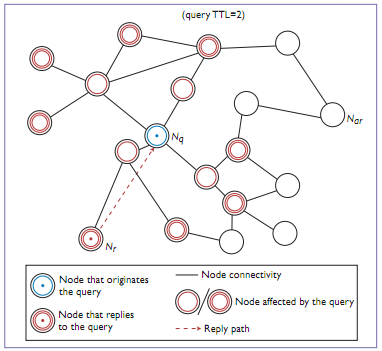
\includegraphics[scale=0.75]{images/flooding-architecture.png}
	\caption{Busca por inundação. O nó azul origina a requisição. Ela trafega pelos outros nós na rede (com circuferências vermelhas) até chegar nó com o conteúdo da requisição que realiza a resposta (com um ponto vermelho no meio). Os nós com três argolas são nós em que o TTL chegou em 0.~\cite{dovalScalable01}.}
	\label{fig:flooding-architecture}
\end{figure}

Essa abordagem porém possui diversas desvantagens. Podemos notar que a probabilidade de congestionamento da rede é muito alta. Diversas requisições de buscas podem ser disparadas por vários nós, o que pode rapidamente sobrecarregar a rede com tantos pedidos. Além disso, mesmo após uma resposta de que o arquivo na rede foi encontrado, as mensagens de requisição continuarão a se propagar na rede. Logo essa abordagem exige uma alta capacidade de processamento, além de exigir muita largura de banda.

Outro problema visível é que não é garantido a disponibilidade de arquivos na rede. Supondo um caso onde um arquivo a ser encontrado está mais longe do que o TTL ou do tempo necessário para encontrá-lo, será impossível para um nó encontrar esse arquivo na rede. Portanto isso ocasionará a indisponibilidade deste arquivo para aquele nó.

Um exemplo de rede que usa a arquitetura de inundação é a \emph{Gnutella}. Ela segue o que foi explicado acima com poucas alterações. Dessa forma características como o anonimato dos peers é bastante comprometida. Além disso, qualquer um pode obter uma lista de arquivos compartilhados de um nó, visto que o \emph{Gnutella} não tem implementações de segurança.

Um outro exemplo pode ser visto na rede \emph{Freenet}, também sem servidor central. De acordo com~\cite{ian02}, o \emph{Freenet} foi desenvolvido para haver o anonimato completo e absoluto. Isso implica que não é possível saber a origem de um arquivo na rede, os nós que estão fazendo download desse arquivo no momento e nem qualquer informação relativa a arquivos. Os objetivos da rede são a liberdade de expressão, liberdade social e política.

A forma de armazenamento da informação é bastante distinta das outras arquiteturas. Um arquivo não fica necessariamente na máquina do usuário, ele pode estar espalhado em máquinas aleatórias pela rede. Quando o número de requisições por esse arquivo cresce, o \emph{Freenet} copia ele para diversos nós na rede. Dessa forma arquivos mais requisitados estão em maiores quantidades na rede. Em contrapartida, arquivos que são menos acessados vão sendo substituídos pelos mais populares, e aos poucos vão sumindo da rede.

Cada arquivo da rede, quando compartilhado, são imediatamente assinados com um certificado digital. Dessa forma o seu conteúdo não pode ser modificado. Por esse motivo e pelo fato de arquivos estarem espalhados pela rede, o usuário de um nó pode não saber que tipo de arquivo está em sua máquina. Dessa forma,um usuário não pode ser responsabilizado pelo conteúdo de sua máquina.

O roteamento de requisições ocorre de forma semelhante ao \emph{Gnutella}, porém a busca por arquivos é feita usando busca em largura, evitando inundação da rede. Além disso quando uma requisição é atendida a resposta volta pelo mesmo caminho da ida.

A rede \emph{Freenet} também realiza \emph{caching}, ou seja, um nó armazena uma lista de arquivos prováveis de estarem armazenados nos vizinhos. Isso aumenta a performance que é bastante reduzida pelo uso de busca em largura.

Uma grande desvantagem do \emph{Freenet} é o seu sistema de busca. Além de possuir as fraquezas da arquitetura de inundação, ela só permite a busca de arquivos pelo nome completo, visto que uma busca por nome parcial poderia identificar o arquivo em um nó e comprometeria o anonimato.


\subsubsection{Redes de sobreposição}

Redes de sobreposição são redes virtuais que são criadas em cima da topologia de rede física. Elas surgem para tentar solucionar o problema de localização de nós e dados na rede sem limitações de alcançe de mensagens, comprometimento do desempenho, centralização de informação e problemas de segurança.

As principais características das redes de sobreposição são:

\begin{itemize}
	\item Auto organizada - A rede gerencia os vizinhos dos nós
	\item Escalável - A entrada ou saída de nós na rede pode ser realizada de maneira fácil.
	\item Descentralização - Não existe uma entidade central que controla informação.
	\item robustez - Não existem ponto único de falhas, entrada e saída de nós não derrubam o sistema, robustez contra ataques.
	\item balanceamento de carga - A rede gerencia os nós com mais processamento para os nós com menos processamento.
\end{itemize}

Atualmente a internet é a base de muitas das redes sobrepostas. Dessa forma é possível rotear mensagens na rede sem a necessidade de endereçar um endereço IP. É possível endereçar nós usando outra forma de identificar um nó, por exemplo tabelas de hash distribuídos.

Tabela de hash distribuídos (DHT) são mecanismos baseados em chave e valor usados para controlar a localização de cada nó na rede. É um mecanismo descentralizado, sem nenhuma forma de coordenação centralizada. Dessa forma eles podem recuperar de forma eficiente um valor na tabela.

Uma característica além da descentralização é a tolerância a falhas das DHTs, elas são confiáveis mesmo com a falha, entrada ou mesmo saída de um nó da rede e garantem o funcionamento da rede em um desses casos.

Diversos algoritmos são implementados com o objetivo de controlar entrada e saída de nós, bem como o roteamento de informações e nós na rede. A próxima seção desse trabalho explica os principais algoritmos das redes de sobreposição, introduzindo conceitos relativos à cada rede.

\subsection{Roteamento}

Segue abaixo os principais algoritmos das redes de sobreposição. O objetivo dessa seção é explicar conceitos introdutórios dos algoritmos, visto que serão importantes para análise de dependabilidade e confiabilidade de entrega de mensagens nos nós. Eles estão estruturados da seguinte forma:
\begin{itemize}
	\item Plaxton
	\item Tapestry
	\item Pastry
	\item Kademlia
	\item Chord
\end{itemize}

\subsubsection{Plaxton}

A rede \emph{Plaxton} consiste em uma estrutura de dados de objetos distribuídos na rede. Ela foi projetada para suportar a localização dos objetos e mensagens para os objetos na rede de forma semelhante ao percorrimento de uma árvore. Em geral uma rede \emph{Plaxton} e todas as outras que foram derivadas dela possuem as seguintes entidades:
\begin{itemize}
	\item \emph{Routers} ou roteadores - São os nós de uma rede \emph{plaxton}.
	\item \emph{Routing} ou roteamento - Troca de mensagens entre os roteadores.
	\item \emph{Publishing} ou publicação - Registro de objetos no nó raiz.
	\item \emph{Plaxton Mesh} - Representa a estrutura de dados da rede.
\end{itemize}

O uso dessa estrutura garante um tempo rápido de entrega das mensagens nos roteadores. Entretanto é importante ressaltar que existem alguns pontos negativos nesse algoritmo. A primeira delas é que a rede é fixa. Ou seja, durante o seu funcionamento não é permitido a inserção ou a remoção de mais nós na rede, visto que um nó será responsável por conhecer todo um caminho e sua ausência implicaria na perda de parte da rede. Além disso, a dere \emph{plaxton} requer a existência de um nó raiz que irá conhecer todos os objetos. Logo a rede possui um ponto único de falha, ou seja, um elemento crítico na rede que caso ocorra uma falha, toda a rede para de funcionar.

O mecanismo de roteamento do \emph{plaxton} cria em cada nó mapas de roteamento locais, também chamados de mapas de vizinhança, que são responsáveis por rotear as mensagens até o seu destino (\emph{destination id}). Esses mapas possuem várias camadas, digamos x camadas, cada uma com um número y de entradas iguais a base do ID. A busca do próximo nó consiste em buscar o próximo dígito do local de destino nos n+1 níveis do mapa uma entrada j em uma camada i.

Esse mecanismo de roteamento permite também uma busca de um objeto no servidor, bem como o envio de mensagens. O servidor que possui o objeto em sua memória faz um anúncio para o nó raiz único na rede, que é responsável por armazenar o endereço de todos os objetos (esse nó único raíz é o ponto único de falha mencionado anteriormente). Essa publicação ao ser enviada para o nó raiz é enviada também para os roteadores que estão no caminho, fazendo então que esses roteadores conheçam quem está abaixo deles.

Como dito anteriormente, é possível o cliente enviar uma mensagem para objetos na rede. Essas mensagens são enviadas para o destinatário de forma a ter como destinatário inicial o nó raiz. A mensagem então vai sendo roteada e caso algum roteador tenha alguma informação do destinatário final da mensagem, ele encaminha então para o mesmo. Caso contrário a mensagem é enviada cada vez mais próxima do nó raiz. Caso a mensagem passe por um caminho onde o nó destinatário não seja conhecido ela será enviada ao nó raiz, onde todos os objetos são registrados. Ela então conhecerá o caminho do nó destinatário final e será roteada até ele.

\subsubsection{Tapestry}

De acordo com~\cite{rowstron01} o \emph{Tapestry} é uma forma de rotear mensagens para o destino de forma eficiente e totalmente descentralizada em um ambiente de carga alta de uso, rede congestionada e alta probabilidade de falha nos nós. O \emph{Tapestry} tem uma noção de localidade dos pares, o que garante que ele conseguirá entregar requisições de forma independente dos nós. Foi desenvolvido em 2004 na Universidade da Califórnia, \emph{Berkley} e foi baseado no \emph{Plaxton}.

O \emph{Tapestry} mantém uma semelhanças com o \emph{Plaxton} que é o modo de endereçamento da malha de vizinhos: O número ID dos vizinhos ainda é o responsável pelo roteamento de mensagens e objetos. Cada vizinho de um nó é separado conforme o número de cada caracter na tabela de vizinhos. Os caracteres do ID normalmente são dígitos hexadecimais, o que ocasiona em uma tabela de base 16, sendo que o \emph{Tapestry} mantém várias tabelas de vizinhos. A tabela~\ref{mapa_vizinhaca_tapestry} exemplifica o que foi mostrado.

\begin{table}
	\caption{Mapa da vizinhança de uma rede \emph{Tapestry}. Caracteres são hexadecimais (base 16), sendo possível até 16 colunas. O número da linha representa o dígito e o número da coluna o valor do caracter na posição do dígito}
	\begin{tabular}{|p{2cm} |p{1cm} |p{1cm} |p{1cm} |p{1cm} |p{1cm} |p{1cm} |p{1cm} |p{1cm}|}
		\hline
		\textbf{Level}	& \textbf{1} & \textbf{2} & \textbf{3}  & \textbf{4}  & \textbf{5}  & \textbf{6} & \textbf{8} & \textbf{A}	\\
		\hline
				1 		& 1D76 		 & 27AB 	  &  			&  			  &		51E5	&	6FA3	 &			  &	            \\
		\hline
				2 		& 	 		 & 		 	  &  43C9		&  	44AF	  &				&			 &			  &	            \\
		\hline
				3 		& 	 		 & 		 	  &  			&  			  &				&			 &			  &	   42A2     \\
		\hline
				4 		& 	 		 & 			  &  			&  			  &				&			 &		4228  &	            \\
		\hline
	\end{tabular}
	\label{mapa_vizinhaca_tapestry}
\end{table}

No mapa da tabela~\ref{mapa_vizinhaca_tapestry}, temos os nós separados por linhas e colunas. Iniciando na primeira linha, podemos verificar que o primeiro dígito de todos os elementos da linha representa o valor correspondente na coluna. Isto é
\begin{itemize}
	\item O primero caracter do registro 1D76 é 1, que corresponde ao valor da sua coluna.
	\item O primero caracter do registro 27AB é 2, que corresponde ao valor da sua coluna.
	\item O primero caracter do registro 51E5 é 5, que corresponde ao valor da sua coluna.
	\item O primero caracter do registro 6FA3 é 6, que corresponde ao valor da sua coluna.
\end{itemize}

O mesmo raciocício se aplica às demais linhas. Por essa tabela, será possível então o roteamento de objetos ao longo da rede. Na imagem~\ref{fig:rede-tapestry}, podemos verificar um roteamento simples de um objeto documento do nó 4228 para o nó 4377 (será omitido por enquanto o mesmo objeto do nó AA93). O primeiro salto de envio verifica o primeiro dígito do \emph{receiver id}, consulta na tabela de vizinhos e faz o envio. No caso, 4228 olha o dígito 1 do id do destino 4377 e em seguida faz o envio para 43FE. Em 43FE ele faz o mesmo procedimento, mas para o segundo dígito do destino 4377. Ele então envia para 437A. O mesmo ocorre para 437 mas para o terceiro dígito do destino 4377. Ele enfim chega no destino 4377 e o objeto pode ser passado para a aplicação.

\begin{figure}
	\centering
	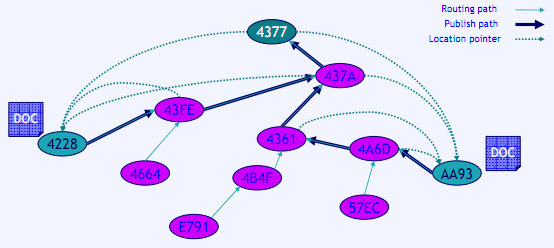
\includegraphics[scale=0.6]{images/rede-tapestry.png}
	\caption{Roteamento de mensagem ou objeto com os ponteiros localizadores do emissor.~\cite{welzi11}}
	\label{fig:rede-tapestry}
\end{figure}

É importante notar aqui algumas características da rede~\emph{Tapestry} que vamos observar na imagem~\ref{fig:rede-tapestry}.

A primeira delas é que na rede podem existir múltiplas cópias do mesmo objeto na rede. Na imagem~\ref{fig:rede-tapestry}, podemos ver que existe o objeto doc com o ID 4377 criado nos nós 4228 e AA93. A segunda característica é a publicação de objetos. Ao longo do roteamento do objeto, mensagens de publicação vão criando \emph{links} do nó atual com o emissor do objeto (representados na figura~\ref{fig:rede-tapestry} pela linha pontilhada). Dessa forma, se uma requisição vier endereçando o nó emissor dito anteriormente, o nó atual irá saber a localização exata do destino devido ao uso do \emph{link} criado anteriormente.

Por exemplo, ainda usando a imagem~\ref{fig:rede-tapestry}, vamos supor uma mensagem saindo do nó 4464 com \emph{receiver id} igual a 4228. O nó irá analisar o primeiro dígito do \emph{receiver id} 4228 e irá enviar ao nó 43FE. O nó olha para o id mensagem chegada e descobre que o seu destino já existe em um link que foi criado anteriormente com a passagem do objeto doc (coincidentemente é o nó anterior, mas poderia ser outros mais distântes). O nó envia então diretamente ao destinatário, sem passar pelos possíveis links do caminho.

A terceira característica é que as vezes podemos ter um nó responsável pelo redirecionamento de objetos/mensagens próximos (endereçam sempre o mesmo destinatário), por exemplo o nó 437A. Esse nó acaba sendo um ponto único de falha, pois sua ausência poderia fragmentar a rede em duas outras redes distintas. O~\emph{Tapestry} então criou uma forma de contornar esse problema: Adicionou vários \emph{roots} responsáveis por esse objeto, de forma a criar vários links. Desta forma, a ausência de um nó não acarretará em problemas.

O~\emph{Tapestry} garante um meio de tolerar falhas na rede. É possível que em ambientes muito dinâmicos e altamente congestionados alguns nós fiquem indisponíveis por certos momentos. Prevendo a indisponibilidade de um nó, essa arquitetura usa uma tabela de vizinhança de outro nó como forma de redundância. Dessa forma será possível destinar mensagens ou objetos a um nó destino mesmo com a ausência de um roteador ausente no caminho.

Além disso, a disponibilidade ou não de um nó é garantida com procedimentos simples do protocolo TCP. O~\emph{Tapestry} faz uso do protocolo TCP enviando sondas para verificar se o nó está disponível ou não. Essas sondas são o TCP Keep Alive, que segundo~\cite{stevens93}, é um mecanismo que envia ou deixa de enviar respostas ICMP caso o host não consiga responder a essa requisição. Se o host estiver indisponível, então o nó passa a usar a redundância até que o nó esteja disponível novamente. Caso não seja possível mais um estabelecimento da conexão, então o host é descartado e outro nó é escolhido para ser uma nova redundância.

Geralmente o~\emph{Tapestry} faz escolhas de nós vizinhos de acordo com parâmetros de proximidade. Por exemplo, um bom parâmetro de proximidade seria o endereço IP, visto que endereços IPs mais próximos poderiam garantir um menor tempo de viagem de pacotes (Round Trip Time - RTT) e possivelmente melhorar a performance da rede.

Existem situações onde o próximo caracter do \emph{receiver id} não existe na tabela de vizinhança do nó. Nesse caso, o~\emph{Tapestry} aplica o ~\emph{Sorrogate Routing}: Deterministicamente o nó irá escolher um próximo elemento na tabela e ele irá avaliar se o id existe ou não neste novo elemento. Caso o novo nó não tenha o id na tabela, um novo nó é eleito até a condição ser aceita. Por exemplo, vamos supor quatro nós: 2716 liga com 4233 que por sua vez liga com 4899 que liga com 4860 que liga-se a uma rede maior. Se uma mensagem de 2716 endereçar 4855, vamos ter a seguinte situação:
\begin{itemize}
	\item O primero caracter do registro 4865 é 4, o nó 2716 irá encaminhar para 4233.
	\item O segundo caracter do registro 4865 é 8, o nó 4233 irá encaminhar para 4899.
	\item O terceiro caracter do registro 4855 é 5, o nó 4899 não tem esse registro na tabela. Um outro valor é deterministicamente eleito. Como a única opção é 6, ele é escolhido. O nó 4899 irá encaminhar para 4860.
	\item O nó 4860 irá realizar o encaminhamento da mensagem.
\end{itemize}

Dessa forma, o~\emph{Tapestry} garante alta disponibilidade da rede sem contudo prejudicar a performance.

\subsubsection{Pastry}

Similar ao~\emph{Tapestry}, o \emph{Pastry} é uma rede de roteamento que também utiliza uma tabela hash distribuída nos seus nós para roteamento. Ela preserva as características da rede~\emph{Tapestry}: É completamente descentralizada, tolerante a falhas, escalável e confiável. A rede \emph{pastry} foi concebida para alto desempenho.

De acordo com~\cite{rowstron01}, a arquitetura \emph{pastry} possui a seguinte característica: Cada nó na rede possui um identificador único(\emph{nodeid}). Ao receber uma mensagem e uma chave numérica, a rede tem a capacidade de realizar o roteamento de forma eficiente para o nó que contém a chave mais próxima numericamente, visando minimizar a viagem da mensagem pela rede.

\begin{figure}
	\centering
	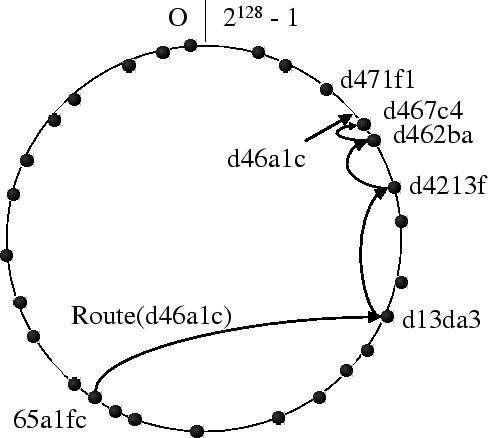
\includegraphics[scale=0.5]{images/roteamento-pastry.png}
	\caption{Roteamento de mensagem na rede pastry do nodo 64a1fc.~\cite{rowstron01}}
	\label{fig:roteamento-pastry}
\end{figure}

A figura~\ref{fig:roteamento-pastry} exemplifica um o roteamento de uma mensagem do nodo 64a1fc até o nodo d467c4. Em cada salto, a rede preocupa-se em encontrar um caminho mínimo para a entrega da mensagem.

O roteamento do \emph{Pastry} possui alguns aspectos interessantes quanto a sua localidade. A rota que uma mensagem deve ser entregue deve ser boa com respeito à métrica de proximidade de nós.

A proximidade, como nas outras redes descritas, está relacionada a uma medida escalar de distância entre dois nós. Assim as propriedades de localidade do \emph{Pastry} são:
\begin{itemize}
	\item Rotas curtas: Prioriza a distância total a ser percorrida. As entradas na tabela de roteamento são referentes ao nó mais próximo. Assim a transmissão de mensagens no nó ocorre sempre no caminho mais curto.
	\item Rotas de convergência: Diz respeito a distância percorrida por duas mensagens enviadas com o mesmo id, antes de suas rota convergirem.
\end{itemize}

\subsubsection{Kademlia}

A arquitetura \emph{Kademlia} foi criada pelos pesquisadores~\emph{Petar Maymounkov e David Mazières}. De acordo com o seu artigo~\cite{maymounkov02}, o \emph{Kademlia} usa DHT para gerênciamento dos pares e possui um número desejavel de características que não estão presentes nas arquiteturas explicadas anteriormente.

Basicamente a arquitetura possui grandes benefícios devido ao uso de uma métrica baseada na operação binária XOR (Ou exclusivo) para medir a distância entre dos nós na rede. Devido ao fator assimétrico, XOR garante ao \emph{Kademlia} saber informações importantes sobre rotas de consultas que ele recebe, além disso construindo tabelas de roteamento rígidas.

O funcionamento do \emph{Kademlia} assemelha-se com o Pastry. Ele trata os nós como folhas em uma árvore binária, dessa forma o percorrimento do nó raiz até uma folha garante um id único para cada nó na rede. A figura~\ref{fig:arvore-kademlia}, que mostra que o percorrimento da raiz até o ponto preto atribui uma chave 0011 ao nó.

Para todos os nós dados, o~\emph{Kademlia} divide a árvore em sucessivas subárvores menores que não contém o nó. A forma da divisão da árvore consiste em:
\begin{itemize}
	\item Dividir a árvore em uma subárvore que conterá metade dos nós da árvore. Essa será a maior subárvore.
	\item Em seguida, dividir em mais uma subárvore que contenha a metade dos nós restantes na árvore.
	\item Proseguir com o método até a divisão completa da árvore.
\end{itemize}
O~\emph{Kademlia} garante que um nó conhece pelo menos um nó em cada uma das subárvores geradas. Dessa forma, é possível a localização de qualquer nó a partir do seu id. Na imagem~\ref{fig:arvore-kademlia} é possível verificar a criação de 4 subárvores: A primeira, com a metade da haste direita do nó raiz (prefixo 1). Em seguida a metade esquerda do nó 0 (prefixo 01). Temos os outros prefixos 0010 e 000.

Conforme dito anteriormente, cada nó na rede possui um identificador único (\emph{nodeId}) de 160 bits, que é gerado aleatóriamente para cada par. As mensagens roteadas pela rede contém junto a si o \emph{nodeId} para que o nó que esteja roteando a mensagem saiba da existência do emissor e grave este \emph{nodeId} caso necessário. As chaves também são 160 bits.

\begin{figure}
	\centering
	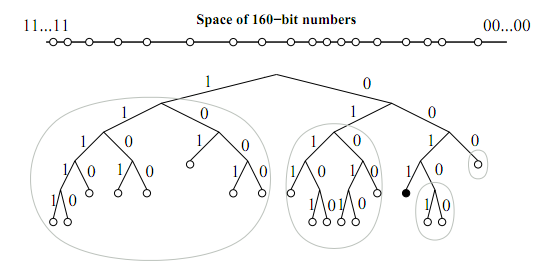
\includegraphics[scale=0.5]{images/arvore-kademlia.png}
	\caption{Árvore binária do \emph{Kademlia} com chaves num espaço de 160 bits. O Ponto preto é o nó 0011, as elipses são os pares que 0011 provavelmente tem contato.~\cite{welzi11}}
	\label{fig:arvore-kademlia}
\end{figure}

Dados dois nós na rede,~\emph{x} e ~\emph{y}, o ~\emph{Kademlia} define a distância desses dois nós como sendo o XOR entre os seus respectivos ~\emph{nodeIds}, ou seja, um valor numérico definido como ~\emph{d(x, y)} =~\emph{x} $\oplus$ \emph{y}.

A operação XOR adiciona algumas características interessantes na rede:
\begin{itemize}
	\item ~\emph{d(x, x)} = 0 e ~\emph{d(x, y)} > 0.
	\item Simetria: ~\emph{d(x, y)} = ~\emph{d(y, x)} para todo \emph{x} diferente de \emph{y}.
	\item Desigualdade do triângulo:~\emph{d(x, y)} +~\emph{d(y, z)} $\ge$ ~\emph{d(x, z)}
\end{itemize}

A operação XOR constrói uma árvore que assemelha-se a um esboço da rede e passa então a distância entre dois nós. Quando uma árvore binária está completa (com o seu tamanho de 160 bits completamente preenchido), a magnitude da distância entre dóis nós pode ser compreendido através da menor subárvore que contém as chaves dos dois nós. Caso a árvore não esteje completa, a noção de distância entre uma folha mais próxima de um id x é o caminho que contém o maior números de dígitos semelhantes a x.

Além disso, o XOR é unidirecional. Dado um ponto \emph{x} e uma distância \emph{d} qualquer, existe um ponto \emph{y} que a sua distância para \emph{x} é exatamente igual a \emph{d}. Isso significa que a busca por uma mesma chave sempre irá convergir em caminhos iguais, independente do nó que originou a busca.

A tabela de roteamento do~\emph{Kademlia} é simples comparado com a dificuldade de balanceamento da árvore binária. Em geral, a tabela consiste em uma árvore binária, com folhas sendo~\emph{k-buckets}. Cada~\emph{k-bucket} cobre uma área de~\emph{nodeId} com prefixo em comum e todos os ~\emph{k-buckets} juntos combrem os 160 bits dos~\emph{nodesIds}.

Na árvore de roteamento, os nós são alocados dinamicamente. Inicialmente a árvore começa vazia. Quando o primeiro nó for inserido na rede, digamos um nó \emph{u}, a árvore terá apenas um \emph{k-bucket} cobrindo todo o espaço da chave de 160 bits.

Quando o nó \emph{u} aprende um novo nó na rede, ele irá tentar colocá-lo na sua tabela de roteamento. De acordo com o seu~\emph{nodeId}, ele irá fazer o posicionamento na árvore. Em seguida tentará inserí-lo na árvore. Se aquele \emph{bucket} não estiver cheio, ele é simplesmete inserido. Caso contrário, o \emph{bucket} é divido em dois outros nós e os seus conteúdos são divididos entre os dois novos nós. Esse processo ocorre repetidamente até a rede ser toda descoberta ou então o limite de 160 bits for completamente preenchido. Caso isso ocorra, um novo nó é simplesmente descartado. A figura~\ref{fig:kademlia-k-bucket} exemplifica todo o processo explicado.

\begin{figure}
	\centering
	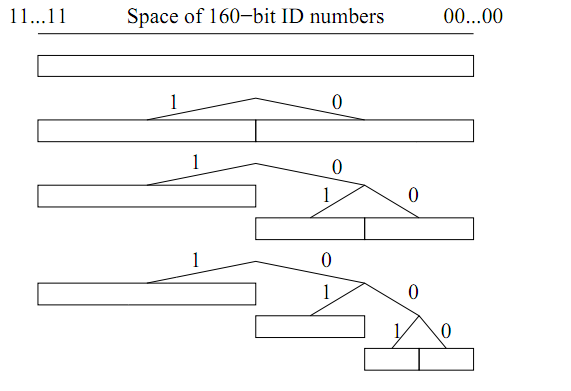
\includegraphics[scale=0.6]{images/kademlia-k-bucket.png}
	\caption{Evolução da árvore binária de roteamento no \emph{Kademlia} com chaves num espaço de 160 bits. Cada novo nó é dividido em um novo \emph{k-bucket}}.
	\label{fig:kademlia-k-bucket}
\end{figure}

Na figura~\ref{fig:kademlia-k-bucket} o primeiro \emph{k-bucket} inserido e ele ocupa os 160 bits. Na linha abaixo, quando um novo nó é descoberto o único \emph{bucket} é divido em outros dois e os seus conteúdos são divididos na rede. Um novo nó \emph{nodeId} de prefixo 00 é encontrado na rede e na linha 3 ele é inserido à direita do nó raiz. Novamente o seus conteúdos são divididos em dois e novos \emph{buckets} são criados. O processo é repetido para cada novo nó na rede.

Como dito anteriormente, uma das dificuldades é o balanceamento da árvore. Caso ocorra a situação, o \emph{Kademlia} tenta contornar isso de forma a manter uma lista com todos os contatos válidos para evitar problemas de notificação dos nós na árvore.

\subsubsection{Chord}

A arquitetura \emph{Chord} define apenas uma operação sobre os nós: O mapeamento sobre os ids. A rede organiza-se na forma de anel, colocando os nós na forma crescente de ID. Sabendo que a rede possui um tamanho de \emph{n} nós, cada nó conhece apenas $\log$(n) vizinhos em sua tabela de roteamento.

Ele basicamente difere-se das outras redes P2P em algumas características. A simplicidade de efetuar rota em cima das chaves, a corretude de necessitar apenas de uma parte correta da informação para garantir a corretude de pesquisas, mapeamento de chaves em nós e não em outros valores. Além disso, necessita de uma pequena quantidade de informação de rota sobre os outros nós.

O protocolo do \emph{Chord} descrito em~\cite{stoica01} espeficica como encontrar a localização das chaves, determina a forma como os nós saem e entram na rede e explica como aplicar algoritmos de estabilização para recuperar nós de falhas nas tabelas de roteamento.

A busca de nós na rede~\emph{Chord} ocorre de maneira muito simples. Ao buscar por um nó de id \emph{x} na rede, a tabela de roteamento é investigada a procura de um ID igual a \emph{x}. Caso não seja encontrado, é feita uma requisição ao nó imediatamente menor que \emph{x}. Esse procedimento é repetido em todos os nós até ser encontrado o nó com id \emph{x} ou então não houverem mais nós menores que \emph{x}.

O \emph{Chord} garante que os resultados de uma pesquisa são corretos mesmo com uma entrada válida na tabela. Como a tabela de roteamento é pequena, é fácil mantê-la atualizada através de algoritmos de estabilização rodando em intervalos regulares.

\section{JAMA}

O desenvolvimento completo da plataforma JAMA está descrita em~\cite{parise11}. Seu objetivo foi desenvolver uma plataforma de sistemas multiagentes distruibuído e com fraco acoplamento entre os agentes e as camadas mais baixas do sistemas, permitindo assim o desenvolvimento de novas funcionalidades. Essa nova plataforma garante a comunicação dos agentes com as outras entidades do ambiente. Atualmente o JAMA está somente com a parte de comunicação de serviços funcional, necessitando de implementação na parte de suporte a agentes.
\begin{itemize}
	\item Tolerância a falhas.
	\item Balanceamento de carga.
	\item Escalabilidade da aplicação.
	\item Descentralização dos serviços nas bordas da rede.
	\item Descentralização de roteamento dos nós.
\end{itemize}


O JAMA foi desenvolvido na linguagem Java e outros frameworks de softwares distrubuidos. Basicamente foi usado tecnologias como o Google Guice (pronunciado juice), que trabalha com injeção de dependências e garante que o código não precise criar objetos diretamente, reduzindo então a dependencia de ``fábricas'' de criações de objetos.

Por se tratar de uma plataforma de sistemas distribuídos, foi necessário escolher um protocolo de rede para a implementação. O protocolo escolhido foi o Peer-to-peer (P2P) pois oferecem uma série de propriedades interessantes para a aplicação:
\begin{itemize}
	\item Tolerância a falhas.
	\item Balanceamento de carga.
	\item Escalabilidade da aplicação.
	\item Descentralização dos serviços nas bordas da rede	.
\end{itemize}

Como foi dito anteriormente, um sistema multiagente tem basicamente duas entidades: Agentes e o ambiente. A plataforma JAMA procurou fazer do ambiente o componente principal no desenvolvimento. Logo a sua arquitetura basicamente preocupou-se com as duas entidades listadas anteriormente e outros dois componentes: Barramento de eventos e um adaptador de rede, visto que é uma aplicação distribuída.

\subsection{Ambiente}

A arquitetura do JAMA atua como uma camada que abstrai as camadas inferiores, permitindo a localização e comunicação de agentes de forma mais transparente. Os agentes emitem mensagens nesse ambiente e ele se encarrega de notificar todos os agentes ouvintes. Por ser uma arquitetura distribuída, os agentes não tem conhecimento se estão rodando na mesma máquina ou não. Logo não existe comunicação direta entre os agentes, o ambiente será o mediador entre eles caso seja necessário haver algum tipo de comunicação. A imagem~\ref{fig:ambiente} sintetiza o que foi explicado.

\begin{figure}
	\centering
	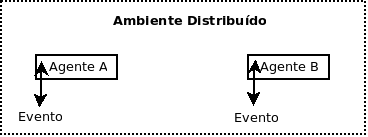
\includegraphics[scale=0.75]{images/ambiente.png}
	\caption{Ambiente distriuído no JAMA. Os agentes não se comunicam diretamente.}
	\label{fig:ambiente}
\end{figure}

O ambiente do JAMA é capaz também de atuar como plataforma provedora de serviços. Aplicações como banco de dados distribuídos, transporte de agentes, e outros podem estar disponíveis na plataforma, bastando apenas serem registrados para serem encontrados pelos agentes. Esses serviços em sua grande maioria são suporte para o processamento dos agentes. Em~\cite{parise11} podemos ver um exemplo de agente que usa aplicações registradas no JAMA:

\begin{quote}
Em aplicações forenses, é muito comum o uso de soluções multiagentes devido ao grande volume de dados e processamento na análise de um caso. Nestas aplicações, o ambiente desempenharia uma função importante ao prover serviços como sistema de arquivos, onde os dados seriam carregados; banco de dados distribuídos, onde os agentes submeteriam seus resultados; e uma aplicação Web, onde os usuários poderiam acompanhar o andamento da análise e executar ações sobre o sistema. Os agentes ficariam com a única responsabilidade de se organizar e executar o trabalho utilizando os serviços fornecidos.
\end{quote}

\subsection{Adaptador de rede}

O Adaptador de rede é responsável por integrar os protocolos de redes ao ambiente. O adaptador de rede deve possuir funcionalidades básicas implementadas para uso da plataforma. Como o JAMA foi projetado para fazer uso de um \emph{middleware open-source} que já implementasse as funcionalidades básicas, não foi necessário fazer uma implementação do início. O \emph{middleware peer-to-peer pastry} foi escolhido para a implementação pois possui bom suporte a segurança, mensagens multicast e boa documentação disponível na internet.

O adaptador é funciona de forma a receber eventos das camadas superiores, serializa os eventos em uma mensagem de rede e envia para a aplicação em algum lugar na rede. Ao receber a mensagem, ela é \emph{desserializada} em um evento e este evento é enviado para as camadas superiores.

\subsection{Barramento de eventos}

O JAMA foi definido para funcionar com o sistema de eventos: Toda e qualquer comunicação entre agentes é feita desta forma. Dessa forma a aplicação não fica acoplada a um tipos específicos de objetos, aumentando assim a escalabilidade da aplicação.

O sistema de eventos está ligado com a definição de evento e ouvintes. Ao montar-se um evento, são passandas todas as informações que forem jugadas necessárias para a comunicação. Em seguida o evento é enviado e a plataforma notifica apenas os ouvintes que estão interessados em receber a comunicação.

O sistema que implementa o despacho e a notificação de eventos é o sistema de barramentos. Seu projeto foi orientado a ser implementado em três padrões de projetos. O primeiro padrão é o \emph{Singleton}, pois o barramento deve ser único na aplicação. O segundo padrão é o \emph{Observer}, pois é nele que se encontram os registros dos ouvintes do sistema e ele irá notifica-los dos eventos enviados. O terceiro padrão é o \emph{Mediator} pois ele atua como mediador da comunicação de elementos da plataforma.

\subsection{Agente}

A parte de agente é responsável por implementar a lógica de sistemas multiagentes. No JAMA, os agentes são executados em paralelo através de Threads separados, sendo responsáveis pelo seu estado e seu fluxo de execução.

O ciclo de vida de um agente segue basicamente os seguintes passos:

\begin{itemize}
	\item \emph{Start} - Ao criar o agente, o ciclo start é iniciado. Normalmente é usado para configurações iniciais do agente.
	\item \emph{Loop} - Código principal que é executado no agente.
	\item \emph{Sleep} - Interrupção da atividade do agente, podendo ser acordado no futuro.
	\item \emph{Wakeup} - Volta para o estado ativo e continua a execução do trecho \emph{loop}.
	\item \emph{Destroy} - Destrói a instância do agente, finalizando a execução.
\end{itemize}


\section{Desafios desse trabalho}
O trabalho porém carece de uma análise de dependabilidade, envolvendo os seus componentes e integração dos mesmos. Não existe um estudo detalhado mensurando o grau de dependabilidade entre os componentes principais (barramento de eventos, adaptador de rede, serviços da rede, etc), nem mesmo detalhando a dependência entre esses módulos.

Além disso, devem ser analisados módulos da rede de sobreposição (o pastry) a fim de garantir alguns aspectos do seu funcionamento. Por exemplo, deve-se analisar a corretude no roteamento das mensagens, ou seja, uma mensagem não vai chegar em um nó ao qual não seja o destino. Também deve ser garantido que as mensagens sempre chegarão ao seu destino, analisando então a robustez do sistema.

O objetivo dessa análise é permitir encontrar pontos onde podem ser melhorados e garantir uma plataforma mais robusta. Dessa forma garantir uma evolução à plataforma Jama que é uma alternativa à plataforma centralizada do observatório web descrito no trabalho~\cite{observatorio}.

O observatório web é um portal para apresentar ao usuário informações relativas à um contexto definido pelo observatório. Essas informações são retiradas de redes sociais, revistas, portais, dentre outros meios de comunicações.

O arcabouço sobre o qual o Observatório foi criado é de forma centralizada, impedido uma escalabilidade e gerando impacto de performance no sistema atual em produção.

Portanto faz-se necessário então um estudo mais aprofundado na plataforma JAMA, sendo esse portanto o foco principal deste trabalho.

























